\section{Enoch's Elevation to Heaven}

\begin{quotex}
When Enoch had lived sixty-five years, he became the father of Methuselah. Enoch walked with God after the birth of Methuselah three hundred years, and had other sons and daughters. Thus all the days of Enoch were three hundred and sixty-five years. Enoch walked with God; and he was not, for God took him. \flright{\textsc{Genesis 5:21-24}}

By faith Enoch was taken up so that he should not see death; and he was not found, because God had taken him. Now before he was taken he was attested as having pleased God. \flright{\textsc{Hebrews 11:5}}

And the same blessing was bestowed upon Ismail and Enoch and Zul-Kifl, because they all practised fortitude. \flright{\textsc{The Prophets, 21:85}}

And remember Enoch in the Book; he was indeed very truthful, a Prophet. And We lifted him to a lofty station. \flright{\textsc{Mary 19:56–57}}

\end{quotex}

Enoch walked with God and was not. That is because he was taken directly up to Heaven without experiencing death. In \emph{The Bezels of Wisdom}, \textbf{Ibn Arabi} describes two ways that the elevation to Heaven can be understood: in terms of place or in terms of rank or degrees.

\begin{quotex}
Elevation has two references — one of place and one of rank. Elevation of place is ``We raised him up to a high place," (19:57) and the highest of places is that upon which the mill of the world of the spheres revolves. It is the sphere of the sun and in it is the station of the spirituality of Enoch, peace be upon him! There are seven heavens under it and seven heavens above it, and it is the fifteenth. That which is above it is the red heaven, i.e., Mars, the heaven of Jupiter, Saturn, the heaven of fixed stars, the Starless Heaven and the heaven of the constellations, the heaven of the Kursi and the heaven of the Arsh. That which is below it is the heaven of Venus, Mercury, the Moon, the circle of ether, the circle of air, the circle of water, and the circle of earth. It is the axis of the heavens, and it is a ``high place".

\end{quotex}

\begin{wrapfigure}{rt}{.3\textwidth}
 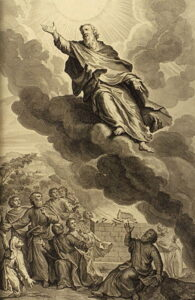
\includegraphics[scale=.5]{a20210529EnochsElevationtoHeaven-img001.jpg} 
 \caption{Enoch's Elevation}
\end{wrapfigure}

\paragraph{Union of Opposites}
Esoteric teaching is nondual, and looks for the common princible that underlies disparate phenomena. That is because God, the ultimate principle of everything existing, is One.

\begin{quotex}
one only has gnosis by joining opposites together in respect of Him. ``He is the First and the Last, the Outwardly Manifest and the Inwardly Hidden." He is the source of what appears and the source of what is hidden in the state of its manifestation. There is none who sees Him other than Him and there is none who is hidden from Him. So He is manifest to Himself and hidden from Himself.

\end{quotex}
Forms in nature may be similar in one respect, yet differ in another. The are both the outward manifestations. Man is in the image of God, and reflects back like a mirror. Mirrors have differing qualities. A purified and cleansed mirror will reflect more precisely than a dusty or smudged mirror. Nevertheless, the Inwardly Hidden is One but the mirrors are multiple.

\begin{quotex}
the world of nature is composed of forms in one mirror. Rather, it is one form in different mirrors.

\end{quotex}
\paragraph{Gnosis and Deeds}
\begin{quotex}
The deed demands place and knowledge demands rank.

\end{quotex}
The exoterics believe that elevation is a place and a reward for their deeds. As a place, there is no place higher than the Throne of God. For the highest degree, there is nothing but God. Elevation is not due to one's essence, but to one's knowledge. Hence, elevation is by rank, not place. Nevertheless, rank, on Earth, is based on authority, whether or not he is worthy of it.

\begin{quotex}
The most knowledgeable of people can be ruled by the person with the position of power, even if that person is the most ignorant of people.

\end{quotex}
His rank has no permanence, and ends with his retirement.

\begin{quotex}
The one with knowledge is not like that.

\end{quotex}
\paragraph{The Heavenly Spheres}
In the \textit{Meditation on Enoch}, Ibn Arabi identifies 15 spheres or ``heavens". The Sun is Enoch's station of spirituality, with seven above it and seven below. The vision is heliocentric, since all the spheres revolve around the Sun. He then discusses whether these spheres refer to ``place" or to degrees of existence. For those rewarded by deeds, they seem to be places. For the gnostic—the man of knowledge—they are degrees of existence.

\begin{enumerate}
\item The Throne (Kursi, `Arsh) (Empyrean) 
\item Zodiac (Primum Mobile) 
\item Starless Heaven (crystalline sphere) 
\item Fixed stars (firmament) 
\item Saturn 
\item Jupiter 
\item Mars 
\item Sun (around which the others revolve) 
\item Venus 
\item Mercury 
\item Moon 
\item Ether 
\item Air 
\item Water 
\item Earth 
\end{enumerate}
Note, too, Dante's description of his Ascent to Heaven.

\flrightit{Posted on 2021-05-29 by Cologero }
